\documentclass[12pt]{article}

% Packages
\usepackage[utf8]{inputenc} % allow utf-8 input
\usepackage[T1]{fontenc}    % use 8-bit T1 fonts
\usepackage{geometry}       % to change the page dimensions
\usepackage{graphicx}       % support the \includegraphics command and options
\usepackage{amsmath}        % for better mathematical formulas
\usepackage{amsfonts}       % for mathematical fonts
\usepackage{amssymb}        % for mathematical symbols
\usepackage{hyperref}       % for hyperlinks
\usepackage{lipsum}         % for generating filler text
\usepackage{float}          % for better figure placement
\usepackage{natbib}         % for better citations
\bibliographystyle{unsrtnat}

% Page geometry
\geometry{a4paper, margin=1in}

\begin{document}

%Title Page
\begin{titlepage}
    \centering
    \vspace*{5cm}

    \Large
    \textbf{Swarm Robotics: Exploration and Mapping in Simulated testing Environments}

    \vspace{1cm}

    Charlie Anthony [candNo: 246537]\\
    Supervisor: Dr Chris Johnson

    \vfill

    \vspace{1cm}

    \small
    Interim report\\
    Computer Science and Artificial Intelligence BSc

    
\includegraphics[width=0.3\linewidth]{sussex_logo.jpg} %Replace 'logo.jpg' with the path to your University of Sussex logo


    \small
    Department of Informatics and Engineering\\
    University of Sussex\\
    November 2023
\end{titlepage}

%Table of Contents
\tableofcontents
\newpage

%Introduction
\section{Introduction}
Swarms exist everywhere in life. Nearly all organisms exhibit some form of swarming behaviours within their
communities. Starlings display impressive organisational behaviour, positioning themselves with respect to the
movement of their neighbours. Humans show swarm behaviours when moving in crowds, for example, moving around sports
venues or exiting buildings in emergencies. No matter how hard you look, regardless if the context, swarms are
typically present.\\
These behaviours can also be artificially created in robotics. Within the realm of computing, parallelising
processes is breaking barrier after barrier - swarm robotics brings the same benefits. Being able to divide and
conquer a problem has the ability to reduce computational complexity by whole orders of magnitude. Therefore, it
would be wasteful not to properly dedicate the time which this discipline deserves.\\
My agents will be placed within close proximity inside a simulated environment and then allowed to explore and
combine their findings; ultimately creating a visualization map of its environment. The agents will need to both
navigate the environment and avoid collisions, whilst creating an internal representation of its surroundings. The
best-case scenario for the swarm I am developing is a fully decentralised system in simulation.\\
I will initially explore this problem by creating SLAM simulations, and then attempting to apply similar techniques
to a centralised system. These initial simulations will employ techniques such as particle filters, loop closures
and [insert something here] in order to create a base-line representation of the environment.

%Professional and Ethical Considerations
\section{Professional and Ethical Considerations}
My project maintains compliance towards all ethical considerations, as there is minimal external involvement from
humans. The majority of my project will be carried out in simulation, therefore no ethical approval is required. Should
my project progress to physically implementing agents, considerations such as safety around the robots, will be considered.
All tests will be carried out in an environment where people cannot be hit, therefore mitigating any trip hazards.\\
Research in this project is within the professional competence of myself, as it significantly relies upon knowledge
obtained from modules such as "Acquired Intelligence and Adaptive Behaviour" and "Fundamentals of Machine Learning." I
will further ensure all relevant gaps in knowledge are explored through reading extensively in the area and communicating
any areas of concern with my supervisor.

%Related Work
\section{Related Work}
\subsection{SLAM}
SLAM (Simultaneous Localisation and Mapping) is a technique used in robotics to create a map of an unknown environment.
It is an important area of research in robotics as it is heavily used in autonomous vehicles, drones and vacuum cleaners;
allowing agents to understand and navigate their environement effectively.\\
SLAM can be broken down into two sub-problems: localisation and mapping. Localisation is the process of determining the
location of a robot in its environment, whilst mapping is the process of constructing a map of the environment. The maps
are constructed using data collected from sensors, such as cameras and laser scanners. A lot of existing work in SLAM is
based on single robot applications, however, there is a growing interest in multi-agent SLAM. One of the greatest
challenges in SLAM is crossing the simulation to reality gap, as in the real world, sensor readings are noisy and
environments are dynamic, which increases the complexity of the problem.

\subsection{Graph-based SLAM}
Graph-based SLAM is a technique used to create a map of an environment, by using a graph to represent the environment. It
works by having a robot move around its environment, whilst taking measurements of its surroundings. These measurements
are usually received by a sensor, such as a camera or laser scanner. The robot then uses these measurements to create a
plot of where objects may be, by combining the measurements from sensors with its memory of the route it has taken. This
technique is used in many applications, such as autonomous vehicles, drones and vacuum cleaners.\\
One limitation of graph-based SLAM is that it is computationally expensive, as it requires a lot of memory to store the
sensor readings. Also, it is not very scalable, as the more sensors that are added, the more memory is required. Another
limitation is that it cannot always be reliable, as the algorithm depends heavily on detecting loop closures, which when
not detected, can lead to a lot of errors in the map. This, combined with even the slightest inaccuracy from sensors/motors
makes it difficult to apply to the real world.

\subsection{Particle Filters}
Another technique used in SLAM is particle filters. Particle filters, also known as Monte Carlo localisation, is a probabalistic
technique used to estimate the localisation of a robot in its environment. It starts with a set of particles randomly distributed
across the environment, which represent possible locations of the robot. Then as the robot moves around the environment, the
particles weights are updated based on the robots sensors. Overall, this technique is very effective, as it is able to localise
the robot in its environment, even when the environment is dynamic. Also, this process is highly parallelisable, as each particle
can be updated independently; which makes this a viable solution for real-world applications. However, particle filters are
susceptible to the "curse of dimensionality", which means that as the number of dimensions increases, the problem's complexity
rapidly increases.

\subsection{Swarm}
Swarm robotics is a discipline which studies the coordination of large numbers of robots. It is largely inspired by biology,
where social organisms achieve complex behaviours through simple interactions with each other and the environment. Swarm
robotics is an important area of research in robotics, as it has many applications, such as search and rescue, exploration
and mapping.\\
One of the benefits of swarm robotics is the scalability and flexibility of the system. This is because the system is
decentralised, meaning that each agent is able to make decisions independently. This allows for repeatability, as the system
can be scaled up or down simply by adding or removing agents. Also, it allows for flexibility, as the system can be adapted
to different environments, as each agent is able to make decisions based on its surroundings.\\
One of the biggest challenges in swarm robotics is the simulation to reality gap. This is because in simulation, the agents
are able to easily share information with each other, whilst in the real world, this is more challenging. Furthermore, swarm
robotics struggles with more complex environments, like outdoors. As a result, swarm robotics still has a lot of room for
research and development.

\subsection{Random Walks}
Random walk exploration in the context of swarm mapping is a technique where agents individually map an environment, using
methods like Graph-based SLAM, Particle Filters, etc. and them combine their findings to a single global map; this is an
example of a centralised system.\\
A example of an implementation of random walk exploration is Brownian motion \cite{brownian_motion}, which is a physics-inspired approach. It works
by applying a random force to each agent, which determines its direction. The agents then move in this direction until they
detect an obstacle, at which point they will change direction. This process is repeated until the environment is fully mapped.
There is randomness provided from the environment, through detecting other agents or obstacles, and randomness in motion, as
each path is determined by a random force. Overall, collective behaviour emerges from these simple rules, which lead to a
global behaviour which efficiently maps an environment.\\
One of the biggest drawbacks of this approach is that it is not scalable, as the agents are not able to communicate their
maps to each other, which can lead to a lot of redundant exploration. This is because equally, sharing their maps with each
other would be very computationally expensive. Also, another limitation is that this approach doesn't guarantee effiency.
This is because of the inherent randomness, which means areas of the environment may be unexplored.\\

%Requirements Analysis
\section{Requirements Analysis}
Table~\ref{tab:requirements_table} shows the requirements for my project, along with their justification.

\begin{table}[H]
    \centering
    \begin{tabular}{|p{0.2\linewidth}|p{0.7\linewidth}|}
        \hline
        \textbf{Requirement} & \textbf{Justification}\\
        \hline
        \textbf{R1} & \textbf{The system must be able to create a map of its environment}\\
        \hline
    \end{tabular}
    \caption{Requirements and their justification}\label{tab:requirements_table}
\end{table}


\section{Project Plan}
\begin{figure}[H]
    \centering
    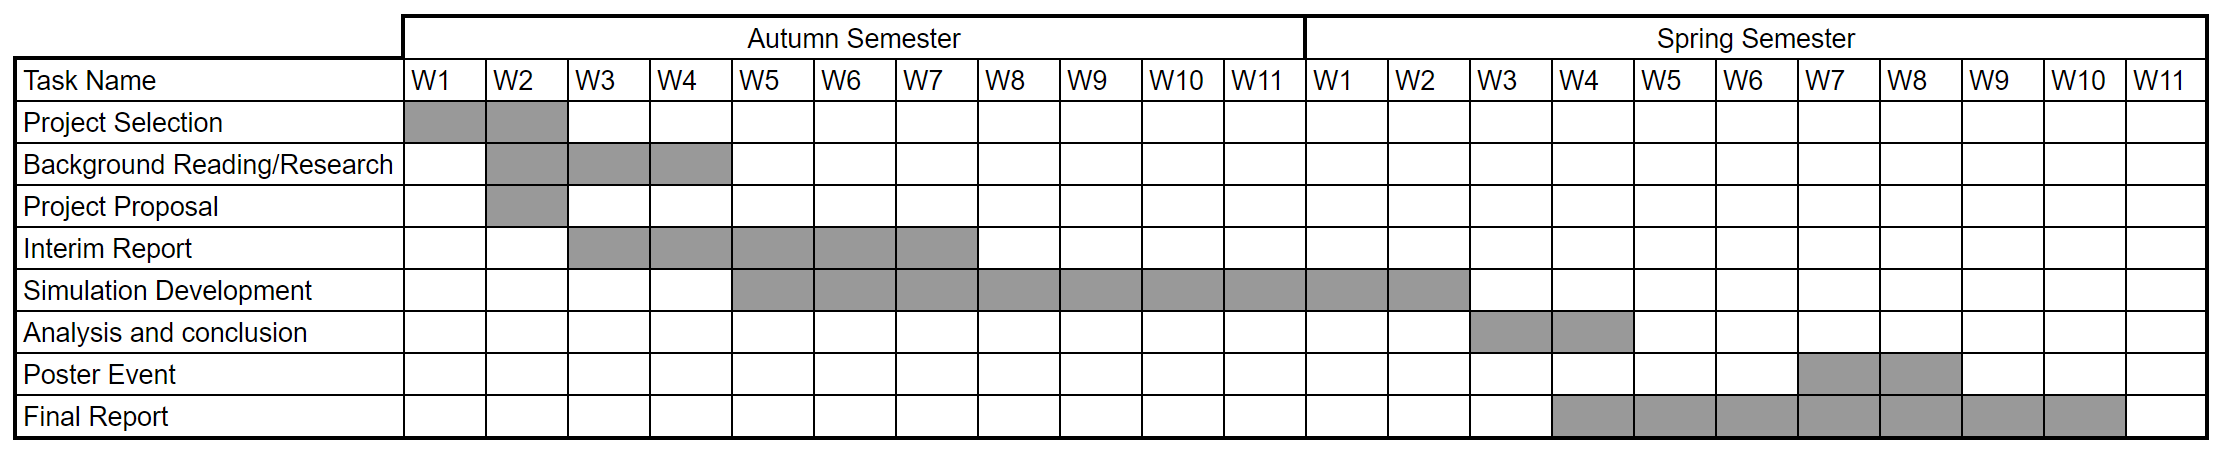
\includegraphics[width=0.8\linewidth]{gantt_chart.png}
    \caption{Gantt chart showing the project plan}
    \label{fig:gantt_chart}
\end{figure}
The execution of my project will be split into various phases, where each phase will focus on an area of development. The
majority of the project will be software development, therefore a large portion time will be spent here. Figure
\ref{fig:gantt_chart} shows the project plan, where the grey bars represent the time spent at each phase.

\section{Methods and Preliminary Results}


\subsection{Supervisor Meetings}

%Appendix
\section{Appendix}

%References
\section{References}

\begin{thebibliography}{9}

    \bibitem{brownian_motion}
    Khmelnitsky, E.
    \textit{Brownian Motion and Swarm Dynamics. In Autonomous Mobile Robots and Multi-Robot Systems, 2019}
    \href{https://doi.org/10.1002/9781119213154.ch12}{https://doi.org/10.1002/9781119213154.ch12}


\end{thebibliography}



\end{document}


